\documentclass[12pt]{article}

%packages
%\usepackage{latexsym}
\usepackage{graphicx}
\usepackage{color}
\usepackage{amsmath}
\usepackage{dsfont}
\usepackage{placeins}
\usepackage{amssymb}
\usepackage{wasysym}
\usepackage{abstract}
\usepackage{hyperref}
\usepackage{etoolbox}
\usepackage{datetime}
\usepackage{xcolor}
\usepackage{alphalph}
\settimeformat{ampmtime}

%\usepackage{pstricks,pst-node,pst-tree}

%\usepackage{algpseudocode}
%\usepackage{amsthm}
%\usepackage{hyperref}
%\usepackage{mathrsfs}
%\usepackage{amsfonts}
%\usepackage{bbding}
%\usepackage{listings}
%\usepackage{appendix}
\usepackage[margin=1in]{geometry}
%\geometry{papersize={8.5in,11in},total={6.5in,9in}}
%\usepackage{cancel}
%\usepackage{algorithmic, algorithm}

\makeatletter
\def\maxwidth{ %
  \ifdim\Gin@nat@width>\linewidth
    \linewidth
  \else
    \Gin@nat@width
  \fi
}
\makeatother

\definecolor{fgcolor}{rgb}{0.345, 0.345, 0.345}
\newcommand{\hlnum}[1]{\textcolor[rgb]{0.686,0.059,0.569}{#1}}%
\newcommand{\hlstr}[1]{\textcolor[rgb]{0.192,0.494,0.8}{#1}}%
\newcommand{\hlcom}[1]{\textcolor[rgb]{0.678,0.584,0.686}{\textit{#1}}}%
\newcommand{\hlopt}[1]{\textcolor[rgb]{0,0,0}{#1}}%
\newcommand{\hlstd}[1]{\textcolor[rgb]{0.345,0.345,0.345}{#1}}%
\newcommand{\hlkwa}[1]{\textcolor[rgb]{0.161,0.373,0.58}{\textbf{#1}}}%
\newcommand{\hlkwb}[1]{\textcolor[rgb]{0.69,0.353,0.396}{#1}}%
\newcommand{\hlkwc}[1]{\textcolor[rgb]{0.333,0.667,0.333}{#1}}%
\newcommand{\hlkwd}[1]{\textcolor[rgb]{0.737,0.353,0.396}{\textbf{#1}}}%

\usepackage{framed}
\makeatletter
\newenvironment{kframe}{%
 \def\at@end@of@kframe{}%
 \ifinner\ifhmode%
  \def\at@end@of@kframe{\end{minipage}}%
  \begin{minipage}{\columnwidth}%
 \fi\fi%
 \def\FrameCommand##1{\hskip\@totalleftmargin \hskip-\fboxsep
 \colorbox{shadecolor}{##1}\hskip-\fboxsep
     % There is no \\@totalrightmargin, so:
     \hskip-\linewidth \hskip-\@totalleftmargin \hskip\columnwidth}%
 \MakeFramed {\advance\hsize-\width
   \@totalleftmargin\z@ \linewidth\hsize
   \@setminipage}}%
 {\par\unskip\endMakeFramed%
 \at@end@of@kframe}
\makeatother

\definecolor{shadecolor}{rgb}{.77, .77, .77}
\definecolor{messagecolor}{rgb}{0, 0, 0}
\definecolor{warningcolor}{rgb}{1, 0, 1}
\definecolor{errorcolor}{rgb}{1, 0, 0}
\newenvironment{knitrout}{}{} % an empty environment to be redefined in TeX

\usepackage{alltt}
\usepackage[T1]{fontenc}

\newcommand{\qu}[1]{``#1''}
\newcounter{probnum}
\setcounter{probnum}{1}

%create definition to allow local margin changes
\def\changemargin#1#2{\list{}{\rightmargin#2\leftmargin#1}\item[]}
\let\endchangemargin=\endlist 

%allow equations to span multiple pages
\allowdisplaybreaks

%define colors and color typesetting conveniences
\definecolor{gray}{rgb}{0.5,0.5,0.5}
\definecolor{black}{rgb}{0,0,0}
\definecolor{white}{rgb}{1,1,1}
\definecolor{blue}{rgb}{0.5,0.5,1}
\newcommand{\inblue}[1]{\color{blue}#1 \color{black}}
\definecolor{green}{rgb}{0.133,0.545,0.133}
\newcommand{\ingreen}[1]{\color{green}#1 \color{black}}
\definecolor{yellow}{rgb}{1,1,0}
\newcommand{\inyellow}[1]{\color{yellow}#1 \color{black}}
\definecolor{orange}{rgb}{0.9,0.649,0}
\newcommand{\inorange}[1]{\color{orange}#1 \color{black}}
\definecolor{red}{rgb}{1,0.133,0.133}
\newcommand{\inred}[1]{\color{red}#1 \color{black}}
\definecolor{purple}{rgb}{0.58,0,0.827}
\newcommand{\inpurple}[1]{\color{purple}#1 \color{black}}
\definecolor{backgcode}{rgb}{0.97,0.97,0.8}
\definecolor{Brown}{cmyk}{0,0.81,1,0.60}
\definecolor{OliveGreen}{cmyk}{0.64,0,0.95,0.40}
\definecolor{CadetBlue}{cmyk}{0.62,0.57,0.23,0}

%define new math operators
\DeclareMathOperator*{\argmax}{arg\,max~}
\DeclareMathOperator*{\argmin}{arg\,min~}
\DeclareMathOperator*{\argsup}{arg\,sup~}
\DeclareMathOperator*{\arginf}{arg\,inf~}
\DeclareMathOperator*{\convolution}{\text{\Huge{$\ast$}}}
\newcommand{\infconv}[2]{\convolution^\infty_{#1 = 1} #2}
%true functions

%%%% GENERAL SHORTCUTS

%shortcuts for pure typesetting conveniences
\newcommand{\bv}[1]{\boldsymbol{#1}}

%shortcuts for compound constants
\newcommand{\BetaDistrConst}{\dfrac{\Gamma(\alpha + \beta)}{\Gamma(\alpha)\Gamma(\beta)}}
\newcommand{\NormDistrConst}{\dfrac{1}{\sqrt{2\pi\sigma^2}}}

%shortcuts for conventional symbols
\newcommand{\tsq}{\tau^2}
\newcommand{\tsqh}{\hat{\tau}^2}
\newcommand{\sigsq}{\sigma^2}
\newcommand{\sigsqsq}{\parens{\sigma^2}^2}
\newcommand{\sigsqovern}{\dfrac{\sigsq}{n}}
\newcommand{\tausq}{\tau^2}
\newcommand{\tausqalpha}{\tau^2_\alpha}
\newcommand{\tausqbeta}{\tau^2_\beta}
\newcommand{\tausqsigma}{\tau^2_\sigma}
\newcommand{\betasq}{\beta^2}
\newcommand{\sigsqvec}{\bv{\sigma}^2}
\newcommand{\sigsqhat}{\hat{\sigma}^2}
\newcommand{\sigsqhatmlebayes}{\sigsqhat_{\text{Bayes, MLE}}}
\newcommand{\sigsqhatmle}[1]{\sigsqhat_{#1, \text{MLE}}}
\newcommand{\bSigma}{\bv{\Sigma}}
\newcommand{\bSigmainv}{\bSigma^{-1}}
\newcommand{\thetavec}{\bv{\theta}}
\newcommand{\thetahat}{\hat{\theta}}
\newcommand{\thetahatmle}{\hat{\theta}_{\mathrm{MLE}}}
\newcommand{\thetavechatmle}{\hat{\thetavec}_{\mathrm{MLE}}}
\newcommand{\muhat}{\hat{\mu}}
\newcommand{\musq}{\mu^2}
\newcommand{\muvec}{\bv{\mu}}
\newcommand{\muhatmle}{\muhat_{\text{MLE}}}
\newcommand{\lambdahat}{\hat{\lambda}}
\newcommand{\lambdahatmle}{\lambdahat_{\text{MLE}}}
\newcommand{\etavec}{\bv{\eta}}
\newcommand{\alphavec}{\bv{\alpha}}
\newcommand{\minimaxdec}{\delta^*_{\mathrm{mm}}}
\newcommand{\ybar}{\bar{y}}
\newcommand{\xbar}{\bar{x}}
\newcommand{\Xbar}{\bar{X}}
\newcommand{\phat}{\hat{p}}
\newcommand{\Phat}{\hat{P}}
\newcommand{\Zbar}{\bar{Z}}
\newcommand{\iid}{~{\buildrel iid \over \sim}~}
\newcommand{\inddist}{~{\buildrel ind \over \sim}~}
\newcommand{\approxdist}{~{\buildrel approx \over \sim}~}
\newcommand{\equalsindist}{~{\buildrel d \over =}~}
\newcommand{\loglik}[1]{\ell\parens{#1}}
\newcommand{\thetahatkminone}{\thetahat^{(k-1)}}
\newcommand{\thetahatkplusone}{\thetahat^{(k+1)}}
\newcommand{\thetahatk}{\thetahat^{(k)}}
\newcommand{\half}{\frac{1}{2}}
\newcommand{\third}{\frac{1}{3}}
\newcommand{\twothirds}{\frac{2}{3}}
\newcommand{\fourth}{\frac{1}{4}}
\newcommand{\fifth}{\frac{1}{5}}
\newcommand{\sixth}{\frac{1}{6}}

%shortcuts for vector and matrix notation
\newcommand{\A}{\bv{A}}
\newcommand{\At}{\A^T}
\newcommand{\Ainv}{\inverse{\A}}
\newcommand{\B}{\bv{B}}
\newcommand{\K}{\bv{K}}
\newcommand{\Kt}{\K^T}
\newcommand{\Kinv}{\inverse{K}}
\newcommand{\Kinvt}{(\Kinv)^T}
\newcommand{\M}{\bv{M}}
\newcommand{\Bt}{\B^T}
\newcommand{\Q}{\bv{Q}}
\newcommand{\Qt}{\Q^T}
\newcommand{\R}{\bv{R}}
\newcommand{\Rt}{\R^T}
\newcommand{\Z}{\bv{Z}}
\newcommand{\X}{\bv{X}}
\newcommand{\Xsub}{\X_{\text{(sub)}}}
\newcommand{\Xsubadj}{\X_{\text{(sub,adj)}}}
\newcommand{\I}{\bv{I}}
\newcommand{\Y}{\bv{Y}}
\newcommand{\sigsqI}{\sigsq\I}
\renewcommand{\P}{\bv{P}}
\newcommand{\Psub}{\P_{\text{(sub)}}}
\newcommand{\Pt}{\P^T}
\newcommand{\Pii}{P_{ii}}
\newcommand{\Pij}{P_{ij}}
\newcommand{\IminP}{(\I-\P)}
\newcommand{\Xt}{\bv{X}^T}
\newcommand{\XtX}{\Xt\X}
\newcommand{\XtXinv}{\parens{\Xt\X}^{-1}}
\newcommand{\XtXinvXt}{\XtXinv\Xt}
\newcommand{\XXtXinvXt}{\X\XtXinvXt}
\newcommand{\x}{\bv{x}}
\newcommand{\onevec}{\bv{1}}
\newcommand{\oneton}{1, \ldots, n}
\newcommand{\yoneton}{y_1, \ldots, y_n}
\newcommand{\yonetonorder}{y_{(1)}, \ldots, y_{(n)}}
\newcommand{\Yoneton}{Y_1, \ldots, Y_n}
\newcommand{\iinoneton}{i \in \braces{\oneton}}
\newcommand{\onetom}{1, \ldots, m}
\newcommand{\jinonetom}{j \in \braces{\onetom}}
\newcommand{\xoneton}{x_1, \ldots, x_n}
\newcommand{\Xoneton}{X_1, \ldots, X_n}
\newcommand{\xt}{\x^T}
\newcommand{\y}{\bv{y}}
\newcommand{\yt}{\y^T}
\renewcommand{\c}{\bv{c}}
\newcommand{\ct}{\c^T}
\newcommand{\tstar}{\bv{t}^*}
\renewcommand{\u}{\bv{u}}
\renewcommand{\v}{\bv{v}}
\renewcommand{\a}{\bv{a}}
\newcommand{\s}{\bv{s}}
\newcommand{\yadj}{\y_{\text{(adj)}}}
\newcommand{\xjadj}{\x_{j\text{(adj)}}}
\newcommand{\xjadjM}{\x_{j \perp M}}
\newcommand{\yhat}{\hat{\y}}
\newcommand{\yhatsub}{\yhat_{\text{(sub)}}}
\newcommand{\yhatstar}{\yhat^*}
\newcommand{\yhatstarnew}{\yhatstar_{\text{new}}}
\newcommand{\z}{\bv{z}}
\newcommand{\zt}{\z^T}
\newcommand{\bb}{\bv{b}}
\newcommand{\bbt}{\bb^T}
\newcommand{\bbeta}{\bv{\beta}}
\newcommand{\beps}{\bv{\epsilon}}
\newcommand{\bepst}{\beps^T}
\newcommand{\e}{\bv{e}}
\newcommand{\Mofy}{\M(\y)}
\newcommand{\KofAlpha}{K(\alpha)}
\newcommand{\ellset}{\mathcal{L}}
\newcommand{\oneminalph}{1-\alpha}
\newcommand{\SSE}{\text{SSE}}
\newcommand{\SSEsub}{\text{SSE}_{\text{(sub)}}}
\newcommand{\MSE}{\text{MSE}}
\newcommand{\RMSE}{\text{RMSE}}
\newcommand{\SSR}{\text{SSR}}
\newcommand{\SST}{\text{SST}}
\newcommand{\JSest}{\delta_{\text{JS}}(\x)}
\newcommand{\Bayesest}{\delta_{\text{Bayes}}(\x)}
\newcommand{\EmpBayesest}{\delta_{\text{EmpBayes}}(\x)}
\newcommand{\BLUPest}{\delta_{\text{BLUP}}}
\newcommand{\MLEest}[1]{\hat{#1}_{\text{MLE}}}

%shortcuts for Linear Algebra stuff (i.e. vectors and matrices)
\newcommand{\twovec}[2]{\bracks{\begin{array}{c} #1 \\ #2 \end{array}}}
\newcommand{\threevec}[3]{\bracks{\begin{array}{c} #1 \\ #2 \\ #3 \end{array}}}
\newcommand{\fivevec}[5]{\bracks{\begin{array}{c} #1 \\ #2 \\ #3 \\ #4 \\ #5 \end{array}}}
\newcommand{\twobytwomat}[4]{\bracks{\begin{array}{cc} #1 & #2 \\ #3 & #4 \end{array}}}
\newcommand{\threebytwomat}[6]{\bracks{\begin{array}{cc} #1 & #2 \\ #3 & #4 \\ #5 & #6 \end{array}}}

%shortcuts for conventional compound symbols
\newcommand{\thetainthetas}{\theta \in \Theta}
\newcommand{\reals}{\mathbb{R}}
\newcommand{\complexes}{\mathbb{C}}
\newcommand{\rationals}{\mathbb{Q}}
\newcommand{\integers}{\mathbb{Z}}
\newcommand{\naturals}{\mathbb{N}}
\newcommand{\forallninN}{~~\forall n \in \naturals}
\newcommand{\forallxinN}[1]{~~\forall #1 \in \reals}
\newcommand{\matrixdims}[2]{\in \reals^{\,#1 \times #2}}
\newcommand{\inRn}[1]{\in \reals^{\,#1}}
\newcommand{\mathimplies}{\quad\Rightarrow\quad}
\newcommand{\mathlogicequiv}{\quad\Leftrightarrow\quad}
\newcommand{\eqncomment}[1]{\quad \text{(#1)}}
\newcommand{\limitn}{\lim_{n \rightarrow \infty}}
\newcommand{\limitN}{\lim_{N \rightarrow \infty}}
\newcommand{\limitd}{\lim_{d \rightarrow \infty}}
\newcommand{\limitt}{\lim_{t \rightarrow \infty}}
\newcommand{\limitsupn}{\limsup_{n \rightarrow \infty}~}
\newcommand{\limitinfn}{\liminf_{n \rightarrow \infty}~}
\newcommand{\limitk}{\lim_{k \rightarrow \infty}}
\newcommand{\limsupn}{\limsup_{n \rightarrow \infty}}
\newcommand{\limsupk}{\limsup_{k \rightarrow \infty}}
\newcommand{\floor}[1]{\left\lfloor #1 \right\rfloor}
\newcommand{\ceil}[1]{\left\lceil #1 \right\rceil}

%shortcuts for environments
\newcommand{\beqn}{\vspace{-0.25cm}\begin{eqnarray*}}
\newcommand{\eeqn}{\end{eqnarray*}}
\newcommand{\bneqn}{\vspace{-0.25cm}\begin{eqnarray}}
\newcommand{\eneqn}{\end{eqnarray}}

%shortcuts for mini environments
\newcommand{\parens}[1]{\left(#1\right)}
\newcommand{\squared}[1]{\parens{#1}^2}
\newcommand{\tothepow}[2]{\parens{#1}^{#2}}
\newcommand{\prob}[1]{\mathbb{P}\parens{#1}}
\newcommand{\cprob}[2]{\prob{#1~|~#2}}
\newcommand{\littleo}[1]{o\parens{#1}}
\newcommand{\bigo}[1]{O\parens{#1}}
\newcommand{\Lp}[1]{\mathbb{L}^{#1}}
\renewcommand{\arcsin}[1]{\text{arcsin}\parens{#1}}
\newcommand{\prodonen}[2]{\bracks{\prod_{#1=1}^n #2}}
\newcommand{\mysum}[4]{\sum_{#1=#2}^{#3} #4}
\newcommand{\sumonen}[2]{\sum_{#1=1}^n #2}
\newcommand{\infsum}[2]{\sum_{#1=1}^\infty #2}
\newcommand{\infprod}[2]{\prod_{#1=1}^\infty #2}
\newcommand{\infunion}[2]{\bigcup_{#1=1}^\infty #2}
\newcommand{\infinter}[2]{\bigcap_{#1=1}^\infty #2}
\newcommand{\infintegral}[2]{\int^\infty_{-\infty} #2 ~\text{d}#1}
\newcommand{\supthetas}[1]{\sup_{\thetainthetas}\braces{#1}}
\newcommand{\bracks}[1]{\left[#1\right]}
\newcommand{\braces}[1]{\left\{#1\right\}}
\newcommand{\set}[1]{\left\{#1\right\}}
\newcommand{\abss}[1]{\left|#1\right|}
\newcommand{\norm}[1]{\left|\left|#1\right|\right|}
\newcommand{\normsq}[1]{\norm{#1}^2}
\newcommand{\inverse}[1]{\parens{#1}^{-1}}
\newcommand{\rowof}[2]{\parens{#1}_{#2\cdot}}

%shortcuts for functionals
\newcommand{\realcomp}[1]{\text{Re}\bracks{#1}}
\newcommand{\imagcomp}[1]{\text{Im}\bracks{#1}}
\newcommand{\range}[1]{\text{range}\bracks{#1}}
\newcommand{\colsp}[1]{\text{colsp}\bracks{#1}}
\newcommand{\rowsp}[1]{\text{rowsp}\bracks{#1}}
\newcommand{\tr}[1]{\text{tr}\bracks{#1}}
\newcommand{\rank}[1]{\text{rank}\bracks{#1}}
\newcommand{\proj}[2]{\text{Proj}_{#1}\bracks{#2}}
\newcommand{\projcolspX}[1]{\text{Proj}_{\colsp{\X}}\bracks{#1}}
\newcommand{\median}[1]{\text{median}\bracks{#1}}
\newcommand{\mean}[1]{\text{mean}\bracks{#1}}
\newcommand{\dime}[1]{\text{dim}\bracks{#1}}
\renewcommand{\det}[1]{\text{det}\bracks{#1}}
\newcommand{\expe}[1]{\mathbb{E}\bracks{#1}}
\newcommand{\expeabs}[1]{\expe{\abss{#1}}}
\newcommand{\expesub}[2]{\mathbb{E}_{#1}\bracks{#2}}
\newcommand{\indic}[1]{\mathds{1}_{#1}}
\newcommand{\var}[1]{\mathbb{V}\text{ar}\bracks{#1}}
\newcommand{\cov}[2]{\mathbb{C}\text{ov}\bracks{#1, #2}}
\newcommand{\corr}[2]{\text{Corr}\bracks{#1, #2}}
\newcommand{\se}[1]{\mathbb{S}\text{E}\bracks{#1}}
\newcommand{\seest}[1]{\hat{\mathbb{S}\text{E}}\bracks{#1}}
\newcommand{\bias}[1]{\text{Bias}\bracks{#1}}
\newcommand{\derivop}[2]{\dfrac{\text{d}}{\text{d} #1}\bracks{#2}}
\newcommand{\partialop}[2]{\dfrac{\partial}{\partial #1}\bracks{#2}}
\newcommand{\secpartialop}[2]{\dfrac{\partial^2}{\partial #1^2}\bracks{#2}}
\newcommand{\mixpartialop}[3]{\dfrac{\partial^2}{\partial #1 \partial #2}\bracks{#3}}

%shortcuts for functions
\renewcommand{\exp}[1]{\mathrm{exp}\parens{#1}}
\renewcommand{\cos}[1]{\text{cos}\parens{#1}}
\renewcommand{\sin}[1]{\text{sin}\parens{#1}}
\newcommand{\sign}[1]{\text{sign}\parens{#1}}
\newcommand{\are}[1]{\mathrm{ARE}\parens{#1}}
\newcommand{\natlog}[1]{\ln\parens{#1}}
\newcommand{\oneover}[1]{\frac{1}{#1}}
\newcommand{\overtwo}[1]{\frac{#1}{2}}
\newcommand{\overn}[1]{\frac{#1}{n}}
\newcommand{\oneoversqrt}[1]{\oneover{\sqrt{#1}}}
\newcommand{\sqd}[1]{\parens{#1}^2}
\newcommand{\loss}[1]{\ell\parens{\theta, #1}}
\newcommand{\losstwo}[2]{\ell\parens{#1, #2}}
\newcommand{\cf}{\phi(t)}

%English language specific shortcuts
\newcommand{\ie}{\textit{i.e.} }
\newcommand{\AKA}{\textit{AKA} }
\renewcommand{\iff}{\textit{iff}}
\newcommand{\eg}{\textit{e.g.} }
\newcommand{\st}{\textit{s.t.} }
\newcommand{\wrt}{\textit{w.r.t.} }
\newcommand{\mathst}{~~\text{\st}~~}
\newcommand{\mathand}{~~\text{and}~~}
\newcommand{\ala}{\textit{a la} }
\newcommand{\ppp}{posterior predictive p-value}
\newcommand{\dd}{dataset-to-dataset}

%shortcuts for distribution titles
\newcommand{\logistic}[2]{\mathrm{Logistic}\parens{#1,\,#2}}
\newcommand{\bernoulli}[1]{\mathrm{Bernoulli}\parens{#1}}
\newcommand{\betanot}[2]{\mathrm{Beta}\parens{#1,\,#2}}
\newcommand{\stdbetanot}{\betanot{\alpha}{\beta}}
\newcommand{\betabinomial}[3]{\text{BetaBinomial}\parens{#1,\,#2,\,#3}}
\newcommand{\multnormnot}[3]{\mathcal{N}_{#1}\parens{#2,\,#3}}
\newcommand{\normnot}[2]{\mathcal{N}\parens{#1,\,#2}}
\newcommand{\classicnormnot}{\normnot{\mu}{\sigsq}}
\newcommand{\stdnormnot}{\normnot{0}{1}}
\newcommand{\uniformdiscrete}[1]{\mathrm{Uniform}\parens{\braces{#1}}}
\newcommand{\uniform}[2]{\mathrm{U}\parens{#1,\,#2}}
\newcommand{\stduniform}{\uniform{0}{1}}
\newcommand{\geometric}[1]{\mathrm{Geometric}\parens{#1}}
\newcommand{\hypergeometric}[3]{\mathrm{Hypergeometric}\parens{#1,\,#2,\,#3}}
\newcommand{\exponential}[1]{\mathrm{Exp}\parens{#1}}
\newcommand{\gammadist}[2]{\mathrm{Gamma}\parens{#1, #2}}
\newcommand{\poisson}[1]{\mathrm{Poisson}\parens{#1}}
\newcommand{\binomial}[2]{\mathrm{Binomial}\parens{#1,\,#2}}
\newcommand{\negbin}[2]{\mathrm{NegBin}\parens{#1,\,#2}}
\newcommand{\rayleigh}[1]{\mathrm{Rayleigh}\parens{#1}}
\newcommand{\multinomial}[2]{\mathrm{Multinomial}\parens{#1,\,#2}}
\newcommand{\gammanot}[2]{\mathrm{Gamma}\parens{#1,\,#2}}
\newcommand{\cauchynot}[2]{\text{Cauchy}\parens{#1,\,#2}}
\newcommand{\invchisqnot}[1]{\text{Inv}\chisq{#1}}
\newcommand{\invscaledchisqnot}[2]{\text{ScaledInv}\ncchisq{#1}{#2}}
\newcommand{\invgammanot}[2]{\text{InvGamma}\parens{#1,\,#2}}
\newcommand{\chisq}[1]{\chi^2_{#1}}
\newcommand{\ncchisq}[2]{\chi^2_{#1}\parens{#2}}
\newcommand{\ncF}[3]{F_{#1,#2}\parens{#3}}

%shortcuts for PDF's of common distributions
\newcommand{\logisticpdf}[3]{\oneover{#3}\dfrac{\exp{-\dfrac{#1 - #2}{#3}}}{\parens{1+\exp{-\dfrac{#1 - #2}{#3}}}^2}}
\newcommand{\betapdf}[3]{\dfrac{\Gamma(#2 + #3)}{\Gamma(#2)\Gamma(#3)}#1^{#2-1} (1-#1)^{#3-1}}
\newcommand{\normpdf}[3]{\frac{1}{\sqrt{2\pi#3}}\exp{-\frac{1}{2#3}(#1 - #2)^2}}
\newcommand{\normpdfvarone}[2]{\dfrac{1}{\sqrt{2\pi}}e^{-\half(#1 - #2)^2}}
\newcommand{\chisqpdf}[2]{\dfrac{1}{2^{#2/2}\Gamma(#2/2)}\; {#1}^{#2/2-1} e^{-#1/2}}
\newcommand{\invchisqpdf}[2]{\dfrac{2^{-\overtwo{#1}}}{\Gamma(#2/2)}\,{#1}^{-\overtwo{#2}-1}  e^{-\oneover{2 #1}}}
\newcommand{\exponentialpdf}[2]{#2\exp{-#2#1}}
\newcommand{\poissonpdf}[2]{\dfrac{e^{-#1} #1^{#2}}{#2!}}
\newcommand{\binomialpdf}[3]{\binom{#2}{#1}#3^{#1}(1-#3)^{#2-#1}}
\newcommand{\rayleighpdf}[2]{\dfrac{#1}{#2^2}\exp{-\dfrac{#1^2}{2 #2^2}}}
\newcommand{\gammapdf}[3]{\dfrac{#3^#2}{\Gamma\parens{#2}}#1^{#2-1}\exp{-#3 #1}}
\newcommand{\cauchypdf}[3]{\oneover{\pi} \dfrac{#3}{\parens{#1-#2}^2 + #3^2}}
\newcommand{\Gammaf}[1]{\Gamma\parens{#1}}

%shortcuts for miscellaneous typesetting conveniences
\newcommand{\notesref}[1]{\marginpar{\color{gray}\tt #1\color{black}}}

%%%% DOMAIN-SPECIFIC SHORTCUTS

%Real analysis related shortcuts
\newcommand{\zeroonecl}{\bracks{0,1}}
\newcommand{\forallepsgrzero}{\forall \epsilon > 0~~}
\newcommand{\lessthaneps}{< \epsilon}
\newcommand{\fraccomp}[1]{\text{frac}\bracks{#1}}

%Bayesian related shortcuts
\newcommand{\yrep}{y^{\text{rep}}}
\newcommand{\yrepisq}{(\yrep_i)^2}
\newcommand{\yrepvec}{\bv{y}^{\text{rep}}}


%Probability shortcuts
\newcommand{\SigField}{\mathcal{F}}
\newcommand{\ProbMap}{\mathcal{P}}
\newcommand{\probtrinity}{\parens{\Omega, \SigField, \ProbMap}}
\newcommand{\convp}{~{\buildrel p \over \rightarrow}~}
\newcommand{\convLp}[1]{~{\buildrel \Lp{#1} \over \rightarrow}~}
\newcommand{\nconvp}{~{\buildrel p \over \nrightarrow}~}
\newcommand{\convae}{~{\buildrel a.e. \over \longrightarrow}~}
\newcommand{\convau}{~{\buildrel a.u. \over \longrightarrow}~}
\newcommand{\nconvau}{~{\buildrel a.u. \over \nrightarrow}~}
\newcommand{\nconvae}{~{\buildrel a.e. \over \nrightarrow}~}
\newcommand{\convd}{~{\buildrel \mathcal{D} \over \rightarrow}~}
\newcommand{\nconvd}{~{\buildrel \mathcal{D} \over \nrightarrow}~}
\newcommand{\withprob}{~~\text{w.p.}~~}
\newcommand{\io}{~~\text{i.o.}}

\newcommand{\Acl}{\bar{A}}
\newcommand{\ENcl}{\bar{E}_N}
\newcommand{\diam}[1]{\text{diam}\parens{#1}}

\newcommand{\taua}{\tau_a}

\newcommand{\myint}[4]{\int_{#2}^{#3} #4 \,\text{d}#1}
\newcommand{\laplacet}[1]{\mathscr{L}\bracks{#1}}
\newcommand{\laplaceinvt}[1]{\mathscr{L}^{-1}\bracks{#1}}
\renewcommand{\min}[1]{\text{min}\braces{#1}}
\renewcommand{\max}[1]{\text{max}\braces{#1}}

\newcommand{\Vbar}[1]{\bar{V}\parens{#1}}
\newcommand{\expnegrtau}{\exp{-r\tau}}

%%% problem typesetting
\definecolor{darkgrey}{rgb}{0.10,0.10,0.9}

\newcommand{\problem}[1]{\noindent \colorbox{black}{{\color{yellow} \large{\textsf{\textbf{Problem \arabic{probnum}}}}~}} \addtocounter{probnum}{1} \vspace{0.2cm} \\ \iftoggle{professormode}{}{\color{darkgrey}} #1}

\newcommand{\easysubproblem}[1]{\ingreen{\item} \iftoggle{professormode}{}{\color{darkgrey}} [easy] #1 \color{black} }
\newcommand{\intermediatesubproblem}[1]{\inorange{\item} \iftoggle{professormode}{}{\color{darkgrey}} [harder] #1 \color{black} }
\newcommand{\hardsubproblem}[1]{\inred{\item} \iftoggle{professormode}{}{\color{darkgrey}} [difficult] #1 \color{black} }
\newcommand{\extracreditsubproblem}[1]{\inpurple{\item} \iftoggle{professormode}{}{\color{darkgrey}} [E.C.] #1 \color{black} }


\newcommand{\spc}[1]{\iftoggle{professormode}{\\ \vspace{#1cm}}{\\ \vspace{-0.3cm}}}

\makeatletter
\newalphalph{\alphmult}[mult]{\@alph}{26}
\renewcommand{\labelenumi}{(\alphmult{\value{enumi}})}

\newcommand{\support}[1]{\text{Supp}\bracks{#1}}
\newcommand{\mode}[1]{\text{Mode}\bracks{#1}}
\newcommand{\IQR}[1]{\text{IQR}\bracks{#1}}
\newcommand{\quantile}[2]{\text{Quantile}\bracks{#1,\,#2}}


\newcommand{\thetahatmap}{\hat{\theta}_{\mathrm{MAP}}}
\newcommand{\thetahatmae}{\hat{\theta}_{\mathrm{MMAE}}}
\newcommand{\thetahatmmse}{\hat{\theta}_{\mathrm{MMSE}}}


\newtoggle{professormode}
% \toggletrue{professormode} %STUDENTS: DELETE or COMMENT this line



\title{MATH 341 / 650.3 Spring 2020 Homework \#8}

\author{Frank Palma Gomez} %STUDENTS: write your name here

\iftoggle{professormode}{
\date{Due by email, Tuesday 11:59PM, May 19, 2020 \\ \vspace{0.5cm} \small (this document last updated \today ~at \currenttime)}
}

\renewcommand{\abstractname}{Instructions and Philosophy}

% !TEX root = ./hw08.tex
\begin{document}
\maketitle

\iftoggle{professormode}{
\begin{abstract}
The path to success in this class is to do many problems. Unlike other courses, exclusively doing reading(s) will not help. Coming to lecture is akin to watching workout videos; thinking about and solving problems on your own is the actual ``working out.''  Feel free to \qu{work out} with others; \textbf{I want you to work on this in groups.}

Reading is still \textit{required}. For this homework set, read about the semi-conjugate normal-inverse-gamma model, grid sampling, Gibbs sampling, and Bayes Factors. Finish the McGrayne book.

The problems below are color coded: \ingreen{green} problems are considered \textit{easy} and marked \qu{[easy]}; \inorange{yellow} problems are considered \textit{intermediate} and marked \qu{[harder]}, \inred{red} problems are considered \textit{difficult} and marked \qu{[difficult]} and \inpurple{purple} problems are extra credit. The \textit{easy} problems are intended to be ``giveaways'' if you went to class. Do as much as you can of the others; I expect you to attempt the \textit{difficult} problems. 

Problems marked \qu{[MA]} are for the masters students only (those enrolled in the 650.3 course). For those in 341, doing these questions will count as extra credit.

This homework is worth 100 points but the point distribution will not be determined until after the due date. See syllabus for the policy on late homework.

Up to 10 points are given as a bonus if the homework is typed using \LaTeX. Links to instaling \LaTeX~and program for compiling \LaTeX~is found on the syllabus. You are encouraged to use \url{overleaf.com}. If you are handing in homework this way, read the comments in the code; there are two lines to comment out and you should replace my name with yours and write your section. The easiest way to use overleaf is to copy the raw text from hwxx.tex and preamble.tex into two new overleaf tex files with the same name. If you are asked to make drawings, you can take a picture of your handwritten drawing and insert them as figures or leave space using the \qu{$\backslash$vspace} command and draw them in after printing or attach them stapled.

The document is available with spaces for you to write your answers. If not using \LaTeX, print this document and write in your answers. I do not accept homeworks which are \textit{not} on this printout. Keep this first page printed for your records.

\end{abstract}

\thispagestyle{empty}
\vspace{1cm}
NAME: \line(1,0){380}
\clearpage
}


\problem{These are questions about McGrayne's book, chapter 17 and the Epilogue.}

\begin{enumerate}

\easysubproblem{What do the computer scientists who adopted Bayesian methods care most about and whose view do they subscribe to? (p233)}
\begin{flushleft}
  They cared about results and they subscribe to John Tukey's view.
\end{flushleft}

\easysubproblem{How was \qu{Stanley} able to cross the Nevada desert?}
\begin{flushleft}
    He moved at an average speed. As the camera took picture, the computer computed the probability of the obstacles. It would take sharp turns and 
    stayed on course most of the time.
\end{flushleft}

\easysubproblem{What two factors are leading to the \qu{crumbling of the Tower of Babel?}}
\begin{enumerate}
    \item Bayes Theorem dependence for the calculation of each individual that has mastered a topic. 
    \item Acumulation of evidence is a survival strategy
\end{enumerate}

\intermediatesubproblem{Does the brain work through iterative Bayesian modeling?}
\begin{flushleft}
    Yes.
\end{flushleft}

\easysubproblem{According to Geman, what is the most powerful argument for Bayesian Statistics?}
\begin{flushleft}
    According to Herman there is no more powerful argument for Bayes thans its recognition of the brains inner structures and prior expectations
\end{flushleft}

\end{enumerate}


\begin{table}[htp]
    \centering
    \small
    \begin{tabular}{l | llll}
    Distribution                  & Quantile  & PMF / PDF  &CDF       & Sampling  \\ 
    of r.v. &  Function & function         & function &  Function \\ \hline
    beta & \texttt{qbeta}($p$, $\alpha$, $\beta$)             
    & \texttt{d-}($x$, $\alpha$, $\beta$)
    & \texttt{p-}($x$, $\alpha$, $\beta$) 
    & \texttt{r-}($\alpha$, $\beta$) \\
    betabinomial & \texttt{qbetabinom}($p$, $n$, $\alpha$, $\beta$)              
    & \texttt{d-}($x$, $n$, $\alpha$, $\beta$)
    & \texttt{p-}($x$, $n$, $\alpha$, $\beta$) 
    & \texttt{r-}($n$, $\alpha$, $\beta$) \\
    
    %betanegativebinomial & \texttt{qbeta\_nbinom}($p$, $r$, $\alpha$, $\beta$) 
    %& \texttt{d-}($x$, $r$, $\alpha$, $\beta$)
    %& \texttt{p-}($x$, $r$, $\alpha$, $\beta$) 
    %& \texttt{r-}($r$, $\alpha$, $\beta$) \\
    
    binomial & \texttt{qbinom}($p$, $n$, $\theta$) 
    & \texttt{d-}($x$, $n$, $\theta$)
    & \texttt{p-}($x$, $n$, $\theta$) 
    & \texttt{r-}($n$, $\theta$) \\
    
    exponential & \texttt{qexp}($p$, $\theta$) 
    & \texttt{d-}($x$, $\theta$) 
    & \texttt{p-}($x$, $\theta$) 
    & \texttt{r-}($\theta$) \\
    
    gamma & \texttt{qgamma}($p$, $\alpha$, $\beta$) 
    & \texttt{d-}($x$, $\alpha$, $\beta$)
    & \texttt{p-}($x$, $\alpha$, $\beta$) 
    & \texttt{r-}($\alpha$, $\beta$) \\
    
    %geometric & \texttt{qgeom}($p$, $\theta$) 
    %& \texttt{d-}($x$, $\theta$)
    %& \texttt{p-}($x$, $\theta$) 
    %& \texttt{r-}($\theta$) \\
    
    inversegamma & \texttt{qinvgamma}($p$, $\alpha$, $\beta$) 
    & \texttt{d-}($x$, $\alpha$, $\beta$)
    & \texttt{p-}($x$, $\alpha$, $\beta$) 
    & \texttt{r-}($\alpha$, $\beta$) \\
    
    negative-binomial & \texttt{qnbinom}($p$, $r$, $\theta$) 
    & \texttt{d-}($x$, $r$, $\theta$) 
    & \texttt{p-}($x$, $r$, $\theta$) 
    & \texttt{r-}($r$, $\theta$) \\
    
    normal (univariate) & \texttt{qnorm}($p$, $\theta$, $\sigma$) 
    & \texttt{d-}($x$, $\theta$, $\sigma$)
    & \texttt{p-}($x$, $\theta$, $\sigma$) 
    & \texttt{r-}($\theta$, $\sigma$) \\
    
    %normal (multivariate) & 
    %& \multicolumn{2}{l}{\texttt{dmvnorm}($\x$, $\muvec$, $\bSigma$)} 
    %& \texttt{r-}($\muvec$, $\bSigma$) \\
    
    poisson & \texttt{qpois}($p$, $\theta$) 
    & \texttt{d-}($x$, $\theta$)
    & \texttt{p-}($x$, $\theta$) 
    & \texttt{r-}($\theta$) \\
    
    T (standard) & \texttt{qt}($p$, $\nu$) 
    & \texttt{d-}($x$, $\nu$) 
    & \texttt{p-}($x$, $\nu$)
    & \texttt{r-}($\nu$) \\
    
    T (nonstandard) & \texttt{qt.scaled}($p$, $\nu$, $\mu$, $\sigma$) 
    & \texttt{d-}($x$, $\nu$, $\mu$, $\sigma$)
    & \texttt{p-}($x$, $\nu$, $\mu$, $\sigma$) 
    & \texttt{r-}($\nu$, $\mu$, $\sigma$) \\
    
    uniform & \texttt{qunif}($p$, $a$, $b$) 
    & \texttt{d-}($x$, $a$, $b$)
    & \texttt{p-}($x$, $a$, $b$) 
    & \texttt{r-}($a$, $b$) \\
    
    
    \end{tabular}
    \caption{Functions from $\texttt{R}$ (in alphabetical order) that can be used on this assignment and exams. The hyphen in colums 3, 4 and 5 is shorthand notation for the full text of the r.v. which can be found in column 2.
    }
    \label{tab:eqs}
    \end{table}

\problem{This problem is about the normal-normal model using a \qu{semi-conjugate} prior. Assume $\Xoneton~|~\theta, \sigsq \iid \normnot{\theta}{\sigsq}$ throughout.}

\begin{enumerate}

\easysubproblem{If $\theta$ and $\sigsq$ are assumed to be independent, how can $\prob{\theta,~\sigsq}$ be factored?}

\begin{align*}
    \prob{\theta,~\sigsq} = \prob{\theta}\prob{\sigsq}  
\end{align*}


\easysubproblem{If $\prob{\theta} = \normnot{\mu_0}{\tausq}$ and $\prob{\sigsq} \sim \invgammanot{\overtwo{n_0}}{\overtwo{n_0 \sigsq_0}}$, find the kernel of the joint posterior, $\cprob{\theta,~\sigsq}{X}$}.

\begin{align*}
    \cprob{\theta,~\sigsq}{X} 
    &= \cprob{X}{\theta,\sigsq}\prob{\theta}\prob{\sigsq}\\
    &= \prod_{i=1}^{n} \normpdf{x_i}{\theta}{\sigsq} \exp{\frac{1}{2\tausq}(\theta - \mu_0)^2}\\
    &\propto (\sigsq)^{-\frac{n}{2}} 
    \exp{-\frac{1}{2\sigsq}((n-1)s^2 + n(\xbar-\theta)^2)} \exp{-\frac{1}{2\tausq}(\theta-\mu_0)^2}
    (\sigsq)^{-\frac{n_0}{2}-1} 
\end{align*}

\hardsubproblem{Show that this kernel can be factored into the kernel of a normal where the leftover is \textit{not} the kernel of an inverse gamma. This is in the lecture notes.}\spc{12}

\begin{align*}
    (\sigsq)^{-\frac{n}{2}} &
    \exp{-\frac{1}{2\sigsq}((n-1)s^2 + n(\xbar-\theta)^2)} \exp{-\frac{1}{2\tausq}(\theta-\mu_0)^2}
    (\sigsq)^{-\frac{n_0}{2}-1}\\
    &\propto (\sigsq)^{-\frac{n}{2}-\frac{n_0}{2}-1} 
    \exp{-\frac{1}{2\sigsq}((n-1)s^2 + n_0\sigsq_0 + n\xbar^2)}
    \exp{(\frac{n\xbar}{\sigsq} + \frac{\mu_0}{\tausq})\theta - ( \frac{n}{2\sigsq} + \frac{1}{\tausq})\theta^2}\\
    &\propto (\sigsq)^{-\frac{n}{2}-\frac{n_0}{2}-1} 
    \exp{-\frac{1}{2\sigsq}((n-1)s^2 + n_0\sigsq_0 + n\xbar^2)}( \frac{n}{2\sigsq} + \frac{1}{\pi})^{-\frac{1}{2}}
    \exp{\frac{(\frac{n\xbar}{\sigsq} + \frac{\mu_0}{\tausq})^2 }{ 4( \frac{n}{2\sigsq} + \frac{1}{2\tausq})}}
\end{align*}

\hardsubproblem{[MA] Find the posterior mode of $\sigsq$ using $k(\sigsq~|~X)$.}\spc{5}

\hardsubproblem{Describe how you would sample from $k(\sigsq~|~X)$. Make all steps explicit and use the notation from Table~\ref{tab:eqs}.}

\begin{enumerate}
    \item Choose $\sigsq_{min}, \sigsq_{max}, \Delta$ to put in  $<\sigsq_{min}, \sigsq_{min} + \Delta, \cdots, \sigsq_{max}>$ 
    \item Compute $C \approx \frac{1}{\sum_{\sigsq \in G} k(\sigsq|X)}$  $ \forall ~ \sigsq_0 \in G$ compute $F(\sigsq_0~|~X) = \prob{\sigsq \leq \sigsq_0~|~X}$
    \item Draw $u$ from $\texttt{runif}(0,1)$ and then put in $X_{samp} = avgmin_{\sigsq \in G} \{ F(\sigsq~|~X) \geq u \}$
    \item Repeat
\end{enumerate}


\hardsubproblem{Describe how you would sample from $\cprob{\theta,~\sigsq}{X}$. Make use of the sampling algorithm in the previous question. Make all steps explicit and use the notation from Table~\ref{tab:eqs}.}
 
\begin{enumerate}
    \item Draw $\sigsq_{samp}$ from $k(\sigsq~|~X)$
    \item Draw $\theta_{samp}$ from $\normnot{\theta}{\sigsq}$
    \item Ship $<\theta_{samp}, \sigsq_{samp}>$ as one sample
    \item Repeat previous steps s times
\end{enumerate}


\hardsubproblem{What are the two main disadvantages of grid sampling?}

\begin{enumerate}
    \item Selecting the the appropriate min, max and $\Delta$.
    \item If $\Delta$ is too small and $dim[\theta]$ is large then it can take infinite time.
\end{enumerate}

\hardsubproblem{Why do you think the prior $\prob{\theta} = \normnot{\mu_0}{\tausq}$ and $\prob{\sigsq} \sim \invgammanot{\overtwo{n_0}}{\overtwo{n_0 \sigsq_0}}$ is called \qu{semi-conjugate}?}

Since both models have their own conjugate models. When you combine two conjugate models you call them semi-conjugate

\extracreditsubproblem{[MA] Find the MMSE of $\sigsq$}\spc{0}

\end{enumerate}

\problem{These are questions which introduce Gibbs Sampling.}

\begin{enumerate}
\easysubproblem{Outline the systematic sweep Gibbs Sampler algorithm below (in your notes).}

\begin{enumerate}
    \item Find reasonable value for  $\theta_0=\theta$
    \item Sample $\sigsq_1$ from $\cprob{\sigsq}{X,\theta}$ where $\theta_0=\theta$
    \item Sample $\theta_1$ from $\cprob{\theta}{X,\sigsq}$ where $\sigsq=\sigsq_1$
    \item Sample  $\sigsq_2$ from $\cprob{\sigsq}{X,\theta}$ where $\theta=\theta_1$
    \item Sample $\theta_2$ from $\cprob{\theta}{X,\sigsq}$ where $\sigsq=\sigsq_2$
    \item Repeat previous steps s times
\end{enumerate}

\extracreditsubproblem{Under what conditions does this algorithm converge?}\spc{0}

\easysubproblem{Pretend you are estimating $\cprob{\theta_1,~\theta_2}{X}$ and the joint posterior looks like the picture below where the $x$ axis is $\theta_1$ and the $y$ axis is $\theta_2$ and darker colors indicate higher probability. Begin at $\bracks{\theta_1,\theta_2} = \bracks{0.5,0.5}$ and simulate 5 iterations of the systematic sweep Gibbs sampling algorithm by drawing new points on the plot (just as we did in class).}


\begin{figure}[htp]
\centering
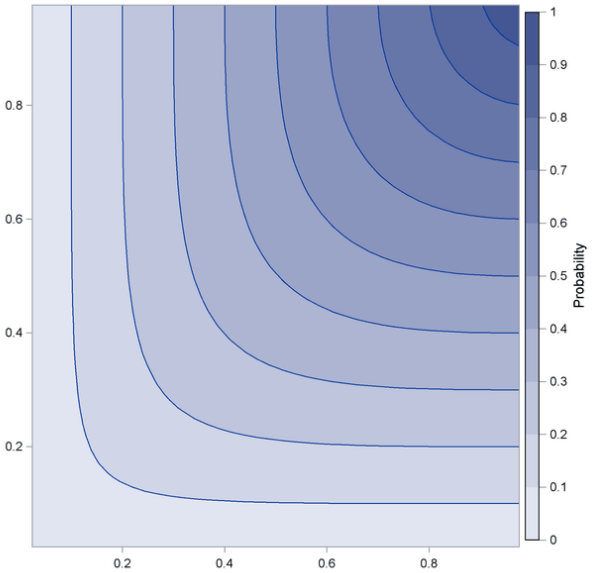
\includegraphics[width=3.5in]{contour.png}
\end{figure}
\end{enumerate}


\problem{These are questions about the change point model and the Gibbs sampler to draw inference for its parameters. You will have to use R to do this question. If you do not have it installed on your computer, you can use R online without installing anything by using a site like \href{https://hub.gke.mybinder.org/user/binder-examples-r-vegj1tni/notebooks/Untitled1.ipynb?kernel_name=ir}{jupyter}. You copy code into the black box and click the \qu{run} button atop. Then you enter more code into the next box and click \qu{run} again, etc.}

\begin{enumerate}

\easysubproblem{Consider the change point Poisson model we looked at in class. We have $m$ exchangeable Poisson r.v.'s with parameter $\lambda_1$ followed by $n-m$ exchangeable Poisson r.v.'s with parameter $\lambda_2$. Both rate parameters and the value of $m$ are unknown so the parameter space is 3-dimensional. Write the likelihood below.}
\begin{align*}
    \cprob{\lambda_1, \lambda_2, m}{x_1, \cdots, x_n}
    &\propto \cprob{x_1, \cdots, x_n}{\lambda_1, \lambda_2, m}\prob{\lambda_1, \lambda_2, m}\\
    &= ( \prod^m_{t=1} \frac{\exp{-\lambda_1}\lambda_1^{x_t}}{x_t!})
    (\prod^n_{t=m+1} \frac{\exp{-\lambda_2}\lambda_2^{x_t}}{x_t!})
    (\frac{1}{n-1})
\end{align*}

\easysubproblem{Consider the model in (a) where $\lambda_1 = 2$ and $\lambda_2 = 4$ and $m=10$ and $n=30$. Run the code on lines 1--14 of the code at the link \href{https://github.com/kapelner/QC_Math_341_Spring_2017/blob/master/lectures/lec20_demos/poisson_gamma_change_pt.R}{here} by copying them from the website and pasting them into an R console. This will plot a realization of the data with those parameters. Can you identify the change point visually?}
\begin{flushleft}
    Approximately 12.
\end{flushleft}


\easysubproblem{Consider the model in (a) but we are blinded to the true values of the parameters given in (b) and we wish to estimate them via a Gibbs sampler. Run the code on lines 16--78 of the code at the link \href{https://github.com/kapelner/QC_Math_341_Spring_2017/blob/master/lectures/lec20_demos/poisson_gamma_change_pt.R}{here} which will run 10,000 iterations. What iteration number do you think the sampler converged?}

\begin{flushleft}
   Approximately 10.   
\end{flushleft}

\easysubproblem{Now we wish to assess autocorrelation among the chains from the Gibbs sampler run in (d). Run the code on lines 79--89 of the code at the link \href{https://github.com/kapelner/QC_Math_341_Spring_2017/blob/master/lectures/lec20_demos/poisson_gamma_change_pt.R}{here}. What do we mod our chains by to thin them out so the chains represent independent samples?}\spc{1}
\begin{flushleft}
    Mod chains to  8
\end{flushleft}

\easysubproblem{Run the code on lines 91--121 of the code at the link \href{https://github.com/kapelner/QC_Math_341_Spring_2017/blob/master/lectures/lec20_demos/poisson_gamma_change_pt.R}{here} which will first burn and thin the chains. Explain these three plots. What distributions do these frequency histograms approximate? You must have $\prob{\text{something}}$ in your answer. What are the blue lines? What are the red lines? What are the grey lines? Read the code if you have to for the answers.}
\begin{itemize}
    \item Histograms are approximations for: $\cprob{\lambda_1}{X_1, \cdots, X_n, \lambda_2, m}, \cprob{\lambda_2}{X_1, \cdots, X_n, \lambda_1, m}$, $\cprob{m}{X_1, \cdots, X_n, \lambda_1, \lambda_2}$.
    \item The blue line represent the best guesss or the means for $\lambda_1 =1.6,\lambda_2 =3.25, m = 9.4$.
    \item The red lines represent the true values where $\lambda_1 =2,\lambda_2 =4, m = 10$.
    \item The grey lines represent the credible regions of $95\%$ where $\lambda_1:[0.7,2.7],\lambda_2:[2.4,4.2], m:[2,19]$.
\end{itemize}

\hardsubproblem{Test the following hypothesis: $H_0: m \leq 15$ by approximating the $p$-value from one of the plots in (e).}
\begin{align*}
    p_{val} &= \cprob{m\leq 15}{X}\\
    &= 0.9597598 > (\alpha = 0.05)
\end{align*}

\hardsubproblem{[M.A.] Explain a procedure to test $H_0: \lambda_1 = \lambda_2$. You can use the plots if you wish, but you do not have to.}

\hardsubproblem{What exactly would come from $\cprob{X^*}{X}$ in the context of this problem? Assume $X^*$ is the same dimension of $X$ (in our toy example, $n=30$). Explain in full detail. Be careful!}
\begin{flushleft}
    Since $\cprob{X^*}{X} = \int_{m} \int_{\lambda_2} \int_{\lambda_1} \cprob{X^*}{\lambda_1, \lambda_2, m} \cprob{\lambda_1, \lambda_2, m}{X} d\lambda_1 d\lambda_2 dm$
    Predicts 31st data point given the estimates of ($\lambda_1, \lambda_2, m$) including previous data.
\end{flushleft}

\extracreditsubproblem{Explain how you would estimate $\cov{\lambda_1}{\lambda_2}$ and what do you think this estimate will be close to?}\spc{7}


\end{enumerate}


\problem{These are questions about the mixture-of-two-normals model and the Gibbs sampler to draw inference for its parameters. You will have to use R to do this question. If you do not have it installed on your computer you can use \href{http://rextester.com/l/r_online_compiler}{this website} which will give you provide you with a workable R console.}

\begin{enumerate}


\easysubproblem{Consider the mixture-of-two-normals model we looked at in class. Write the likelihood below.}\spc{4}

\begin{align*}
    \prob{\theta_1, \sigsq_1, \theta_2, \sigsq_2, ~\rho} &= \prod_{i=1}^{n} (\rho \frac{1}{\sqrt{2\pi\sigsq_1}}\exp{-\frac{1}{2\sigsq_1} \squared{x_i-\theta_1}} + (1 - \rho) \frac{1}{\sqrt{2\pi\sigsq_2}}\exp{-\frac{1}{2\sigsq_2}\squared{x_i-\theta_2}})
\end{align*}

\easysubproblem{Consider the model in (a) with $\theta_1 = 0,~\theta_2 =4,~\sigsq_1 = 2,~\sigsq_2 = 1$ and $\rho = 2$. These are the targets of inference so pretend you don't know their values! Run the code on lines 1--16 of the code at the link \href{https://github.com/kapelner/QC_Math_341_Spring_2017/blob/master/lectures/lec21_demos/mixture_model/mixture_model_gibbs.R}{here} by copying them from the website and pasting them into an R console. This will plot a realization of the data with those parameters. Can you identify that it's a mixture of two normals visually?}\spc{1}

   Yes since there are two humps. Some will samples belong to the first and some to the second one. 

\easysubproblem{Consider the model in (a) but we are blinded to the true values of the parameters given in (b) and we wish to estimate them via a Gibbs sampler. Run the code on lines 19--92 of the code at the link \href{https://github.com/kapelner/QC_Math_341_Spring_2017/blob/master/lectures/lec21_demos/mixture_model/mixture_model_gibbs.R}{here} which will run 10,000 iterations. What iteration number do you think the sampler converged?}\spc{1}

    Iteration number of about 50

\easysubproblem{Now we wish to assess autocorrelation among the chains from the Gibbs sampler run in (d). Run the code on lines 96--103 of the code at the link \href{https://github.com/kapelner/QC_Math_341_Spring_2017/blob/master/lectures/lec21_demos/mixture_model/mixture_model_gibbs.R}{here}. What do we mod our chains by to thin them out so the chains represent independent samples?}\spc{3}


    We can modify the thinning, include more samples, or more iterations. 

\easysubproblem{Run the code on lines 120--152 of the code at the link \href{https://github.com/kapelner/QC_Math_341_Spring_2017/blob/master/lectures/lec21_demos/mixture_model/mixture_model_gibbs.R}{here} which will first burn and thin the chains. Explain these five plots. What distributions do these frequency histograms approximate?}\spc{4}

    The blue line represents the best guess for each of the five parameters. These distograms approximate the normal distribution. 

\hardsubproblem{Provide and approximate $CR_{\rho, 95\%}$. Does it capture the true value of $\rho$?}\spc{4}

    \begin{align*}
        \text{CR}_{\rho, 95\%} &= [0.235, 0.375] \text{, It does not capture $\rho$}
    \end{align*}

\hardsubproblem{Explain carefully how you would approximate $\cprob{X^*}{X}$.}\spc{4}


\hardsubproblem{Explain carefully how you would approximate the probability that the 17th observation belonged to the $\normnot{\theta_1}{\sigsq_1}$ distribution.}\spc{4}

    Take th expectation of the best guess. With that you can see the probability if the 17th observation belongs to $\normnot{\theta_1}{\sigsq_1}$

\easysubproblem{If one of the $\theta$'s did not have a known conditional distribution, which algorithm could you use? Would this algorithm take longer or shorter to converge than the Gibbs sampler you've seen here?}\spc{3}

    You could use grid sampling. This algorithm would take longer to converge. 

\extracreditsubproblem{Explain carefully how you would test if $\theta_1 \neq \theta_2$.}\spc{4}

\end{enumerate}

\problem{This question is about a famous  extra sensory perception (ESP) experiment.}

\begin{figure}[htp]
\centering
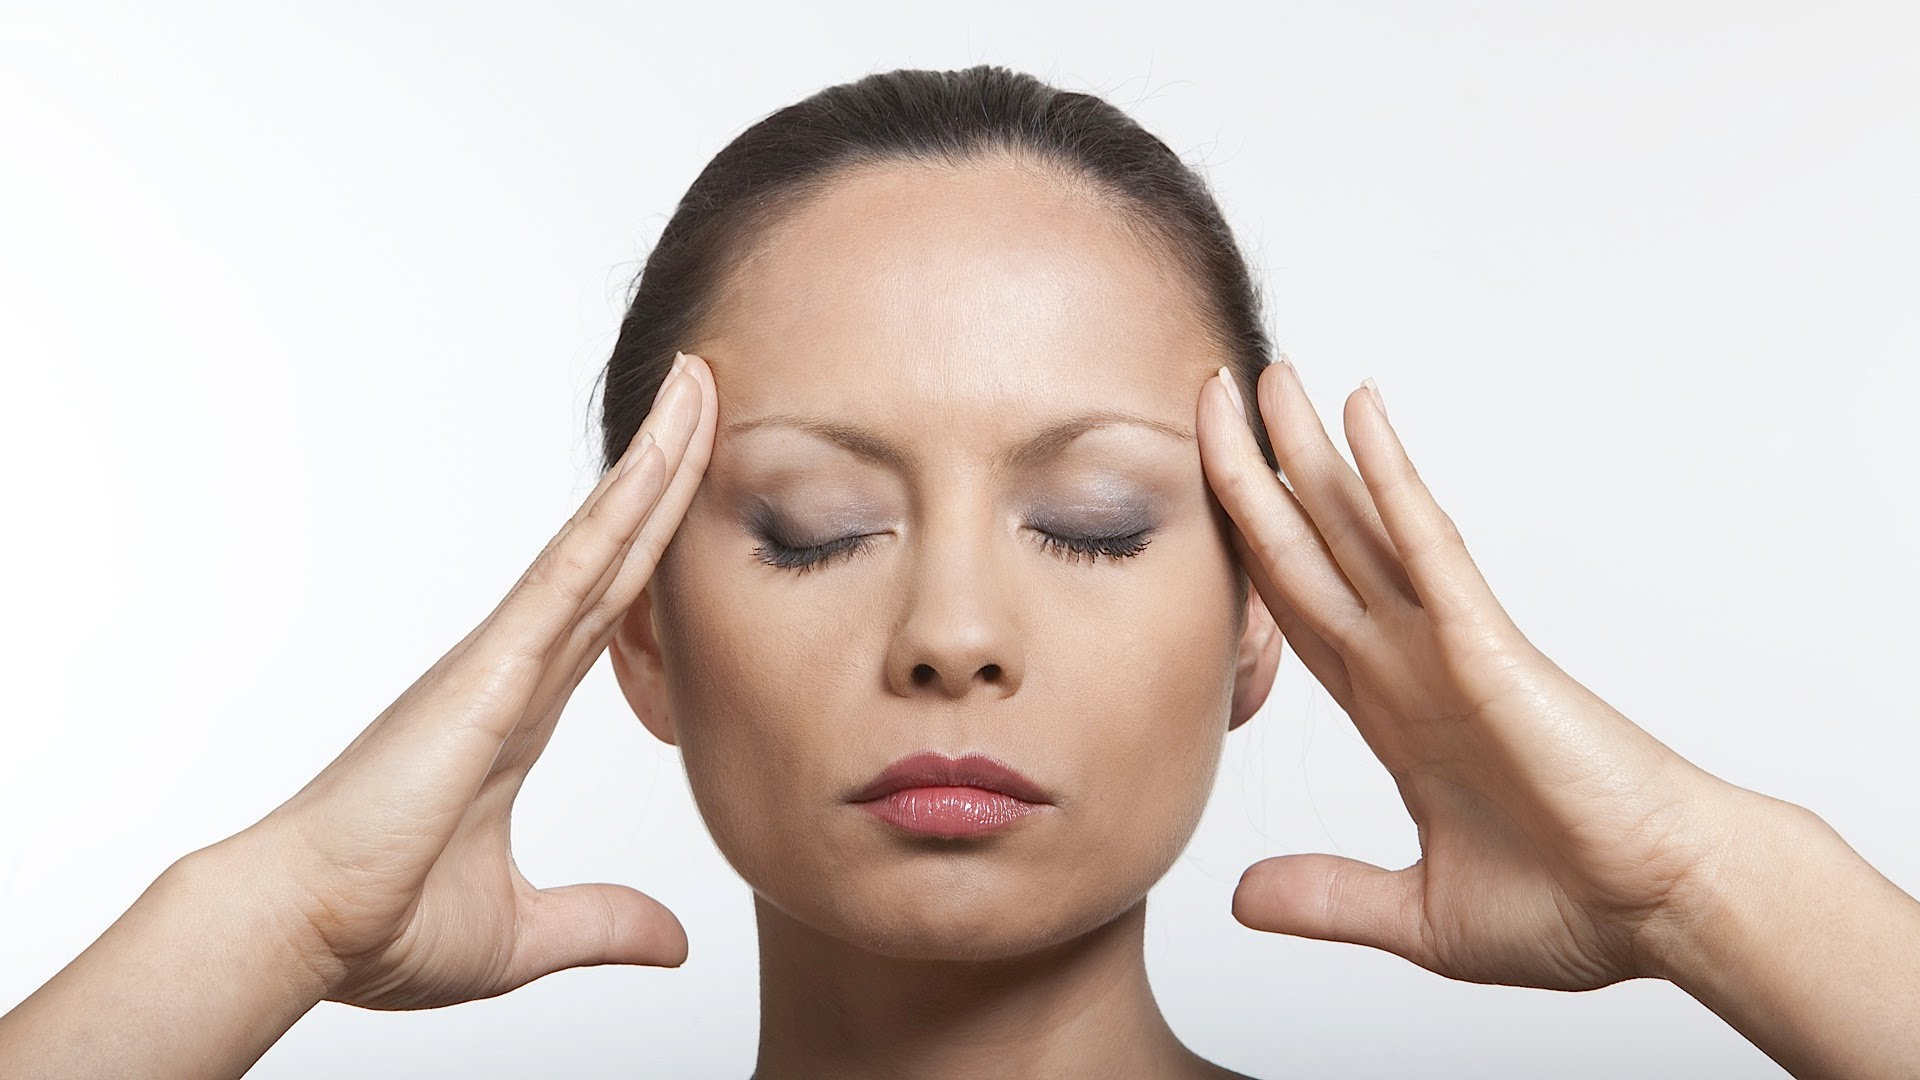
\includegraphics[width=2.8in]{esp.jpg}
\end{figure}

According to quantum mechanics, an event should happen with exactly probability 50\%. So if someone comes with a claim that they have ESP and can affect this event with their mind, then the event no longer has probability 50\% (this is what we are trying to prove).

An experiment was run with someone claiming they have ESP. They tried to affect the event with their mind. The data is as follows: of $n= 104,490,000$ observations, the number of events was $x = 52,263,970$. We will now test to see if the person has ESP a number of ways and try to reconcile the differences.

\begin{enumerate}

\easysubproblem{What is the MLE for the probability of the event?}\spc{1}

\begin{align*}
    \thetahatmmse = \xbar = \frac{1}{n} \sum x_i = 0.5001
\end{align*}

\easysubproblem{Run a two-sided frequentist test at $\alpha = 5\%$ and report the decision (i.e. retain or reject) and the $p$ value.}\spc{2}

\begin{align*}
    \text{RR} &= [0.5 ~\pm~ 2\sqrt{\frac{0.5(1-0.5)}{104, 490, 000}}] = [0.49, 0.50] \\ 
    \text{H}_0 &: \theta = 0.5 \\ 
    \text{H}_a &: \theta \neq 0.5 \\ 
    \theta &\in \text{RR}_{\theta, 95\%} \text{ Retain $H_0$ } \\ 
    P_{val} &= 0.003 < \alpha = 0.5
\end{align*}

\intermediatesubproblem{Run a two-sided Bayesian test assuming the principle of indifference. Use the equivalence region approach with $\delta = 0.01$. Report the decision (i.e. retain or reject) and the $p$ value.}\spc{3}

\begin{align*}
    \text{H}_0 &: \theta = 0.5 \\ 
    \text{H}_a &: \theta \neq 0.5 \\ 
   \text{CR}_{\theta, 95\%} &= [\text{qbeta}(0.025, x + 1, n - x + 1), \text{qbeta}(0.975, x+1, n-x+1)] \\ 
    &= [0.50008567, 0.5002774]
\end{align*}

Ratain $H_0$ since $\theta \in $ CR$_{\theta, 95\%}$ 

\hardsubproblem{Calculate the Bayes Factor $B$ where the alternative hypothesis of $\theta \neq 0.5$ can be summed up with $\theta \sim \stduniform$.}\spc{6}

\begin{align*}
    \text{H}_0 &: \theta = 0.5 \\ 
    \text{H}_a &: \theta \neq 0.5 \\ 
    \alpha &= 5\% \\ 
    \text{B} &= \frac{\text{B}(52,263,971, ~52,226,031)}{(0.5)^{104, 490, 000}} \\
    &\approx 0.33
    % \text{B} &= \text{B}
\end{align*}

Retain $H_0$ 



\hardsubproblem{Try to reconcile parts (b), (c), (d), (e). Why are there different answers? What is going on??}\spc{6}

    With the frequentist pval, bayesian pval, and Bayes Factor B we access "statistical significance". We could also messure "clinical significance", how important the actual effect of theta is. 
    Bayes factors puts both of these ideas together. 

\end{enumerate}

\end{document}


%%%%%%%%%%%%%%%%%%%%%%%%%%%%%%



\end{document}


\problem{These are questions about McGrayne's book, chapter 16.}

\begin{enumerate}
\easysubproblem{What was the main problem facing Bayesian Statistics in the early 1980's?}\spc{4}

\intermediatesubproblem{What is the \qu{curse of dimensionality?}}\spc{4}

\easysubproblem{How did Bayesian Statistics help sociologists?}\spc{4}

\easysubproblem{How did Gibbs sampling come to be?}\spc{3}

\easysubproblem{Were the Geman brothers the first to discover the Gibbs sampler?}\spc{4}

\easysubproblem{Who officially discovered the expectation-maximization (EM) algorithm? And who \textit{really} discovered it?}\spc{4}

\intermediatesubproblem{How did Bayesians \qu{break} the curse of dimensionality?}\spc{4}

\intermediatesubproblem{Consider the integrals we use in class to find expectations or to approximate PDF's / PMF's --- how can they be replaced?}\spc{4}

\easysubproblem{What did physicists call \qu{Markov Chain Monte Carlo} (MCMC)? (p222)}\spc{1}

\easysubproblem{Why is sampling called \qu{Monte Carlo} and who named it that?}\spc{4}

\easysubproblem{The Metropolis-Hastings (MH) Algorithm is world famous and used in myriad applications. Why didn't Hastings get any credit?}\spc{4}

\easysubproblem{The combination of Bayesian Statistics + MCMC has been called ... (p224)}\spc{1}


\extracreditsubproblem{p225 talks about Thomas Kuhn's ideas of \qu{paradigm shifts.} What is a \qu{paradigm shift} and does Bayesian Statistics + MCMC qualify?}\spc{8}

\easysubproblem{How did the \href{http://www.mrc-bsu.cam.ac.uk/software/bugs/}{BUGS} software change the world?}\spc{4}

\easysubproblem{Lindley said that Bayesian Statistics would win out over Frequentist Statistics because it was more logical. What in reality was the reason for the eventual victory of Bayes?}\spc{4}

\extracreditsubproblem{One of my PhD advisors, \href{https://statistics.wharton.upenn.edu/profile/563/}{Ed George} at Wharton told me that \qu{Bayesian Statistics is really `knowledge engineering.'} Is this true? Explain.}\spc{3}

\extracreditsubproblem{Take a look at the software \href{http://mc-stan.org/}{Stan}. What kind of potential does it have to change the world? Note: I had an opportunity to work on Stan as a postdoc (right after I finished his PhD) but chose to come to QC instead.}\spc{10}

\end{enumerate}







\problem{Now we will move to the Bayesian normal-normal model for estimating both the mean and variance and demonstrate similarities with the classical results.}

\begin{enumerate}

\intermediatesubproblem{If $\Xoneton~|~\theta, \sigsq \iid \normnot{\theta}{\sigsq}$ and $X$ represents all $\Xoneton$, Find the kernel of $\cprob{\theta,~\sigsq}{X}$ if $\prob{\theta,~\sigsq} \propto \oneover{\sigsq}$. Use the substitution that we made in class:

\beqn
\sum_{i=1}^n (x_i - \theta)^2 = (n-1)s^2 + n(\xbar - \theta)^2
\eeqn

where $s^2 := \oneover{n-1} \sum_{i=1}^n (x_i -\xbar)^2$. We do this here because this substitution is important for what comes next.}\spc{8}


\intermediatesubproblem{Using Bayes Rule, break up $\cprob{\theta,~\sigsq}{X}$ into two pieces. How are those two pieces distributed?}\spc{6}

\intermediatesubproblem{Using your answer from (b), explain in English how you can create samples from the distribution $\cprob{\theta,~\sigsq}{X}$ that look like $\braces{\bracks{\theta_1, \sigsq_1}, \bracks{\theta_2, \sigsq_2}, \ldots, \bracks{\theta_S, \sigsq_S}}$.}\spc{8}

\hardsubproblem{Using these samples, how would you estimate $\cexpe{\theta}{X}$ and $\cexpe{\sigsq}{X}$? Why is $\cexpe{\theta}{X}$ of paramount importance?}\spc{5}


\hardsubproblem{Using these samples, how would you estimate a 95\% CR for $\theta$?}\spc{5}

\hardsubproblem{Using these samples, how would you obtain a $p$-val for testing if $\sigsq > 1.364$?}\spc{5}

\hardsubproblem{[MA] Using these samples, how would you estimate $\corr{\theta~|~X}{~\sigsq~|~X}$ i.e. the correlation between the posterior distributions of the two parameters?}\spc{3}

%\easysubproblem{If $\Xoneton~|~\theta, \sigsq \iid \normnot{\theta}{\sigsq}$ and $\theta \sim \normnot{\mu_0}{\tausq}$ write the distribution of $\theta~|~X,\sigsq$. Hint: it's in the notes and it was HW6 6(d). Note this problem is independent of the other problems.}\spc{5}

\easysubproblem{Find $\cprob{\theta}{X,~\sigsq}$ by using the full posterior kernel from (a) and then conditioning on $\sigsq$. You should get the same answer as we did before the midterm.}\spc{3}

\easysubproblem{Find $\cprob{\sigsq}{X,~\theta}$ by using the full posterior kernel from (a)  and then conditioning on $\theta$. You should get the same answer as we did before the midterm.}\spc{4}

%\intermediatesubproblem{Show that $\cprob{\sigsq}{X}$ is an inverse gamma distribution and find its parameters.}\spc{4}

\hardsubproblem{Show that $\cprob{\theta}{X}$ is a non-standard $T$ distribution and find its parameters. Assume the prior $\prob{\theta,~\sigsq} \propto \oneover{\sigsq}$. The answer is in the notes, but try to do it yourself.}\spc{15}


\hardsubproblem{Show that $\cprob{\sigsq}{X}$ is an inverse gamma and find its parameters. Assume the prior $\prob{\theta,~\sigsq} \propto \oneover{\sigsq}$. The answer is in the notes, but try to do it yourself.}\spc{12}


%\intermediatesubproblem{How does this compare to 2(j)? Note that $X \sim \invgammanot{\alpha}{\beta}$ then $cX \sim \invgammanot{\alpha}{\frac{\beta}{c}}$.}\spc{2}

\easysubproblem{Write down the distribution of $\cprob{X^*}{X}$ assuming the prior $\prob{\theta,~\sigsq} \propto \oneover{\sigsq}$. This is in the notes.}\spc{1}

\extracreditsubproblem{Prove what you wrote in the previous question: $\cprob{X^*}{X}$ is the non-standard $T$ distribution and find its parameters.}\spc{0}


\intermediatesubproblem{Explain how to sample from the distribution of $\cprob{X^*}{X}$. Also in the notes.}\spc{9}

\intermediatesubproblem{Now consider the informative conjugate prior of $\prob{\theta,~\sigsq} = \cprob{\theta}{\sigsq} \prob{\sigsq}$ where $\cprob{\theta}{\sigsq} = \normnot{\mu_0}{\frac{\sigsq}{m}}$ and $\prob{\sigsq} = \invgammanot{\overtwo{n_0}}{\overtwo{n_0 \sigsq_0}}$ i.e. the general normal-inverse-gamma. What is its kernel? Collect common terms and be neat.}\spc{9}


\hardsubproblem{[MA] If $\Xoneton~|~\theta, \sigsq \iid \normnot{\theta}{\sigsq}$ and given the general prior above, find the posterior and demonstrate it that the normal-inverse gamma is conjugate for the normal likelihood with both mean and variance unknown. This is what I did \emph{not} do in class.}\spc{13}

\end{enumerate}

\problem{We model the returns of S\&P 500 here.}

\begin{enumerate}
\easysubproblem{Below are the 16,428 daily returns (as a percentage) of the S\&P 500 dating back to January 4, 1950 and the code used to generate it. Does the data look normal? Yes/no}\spc{0}

\begin{figure}[h]
\centering
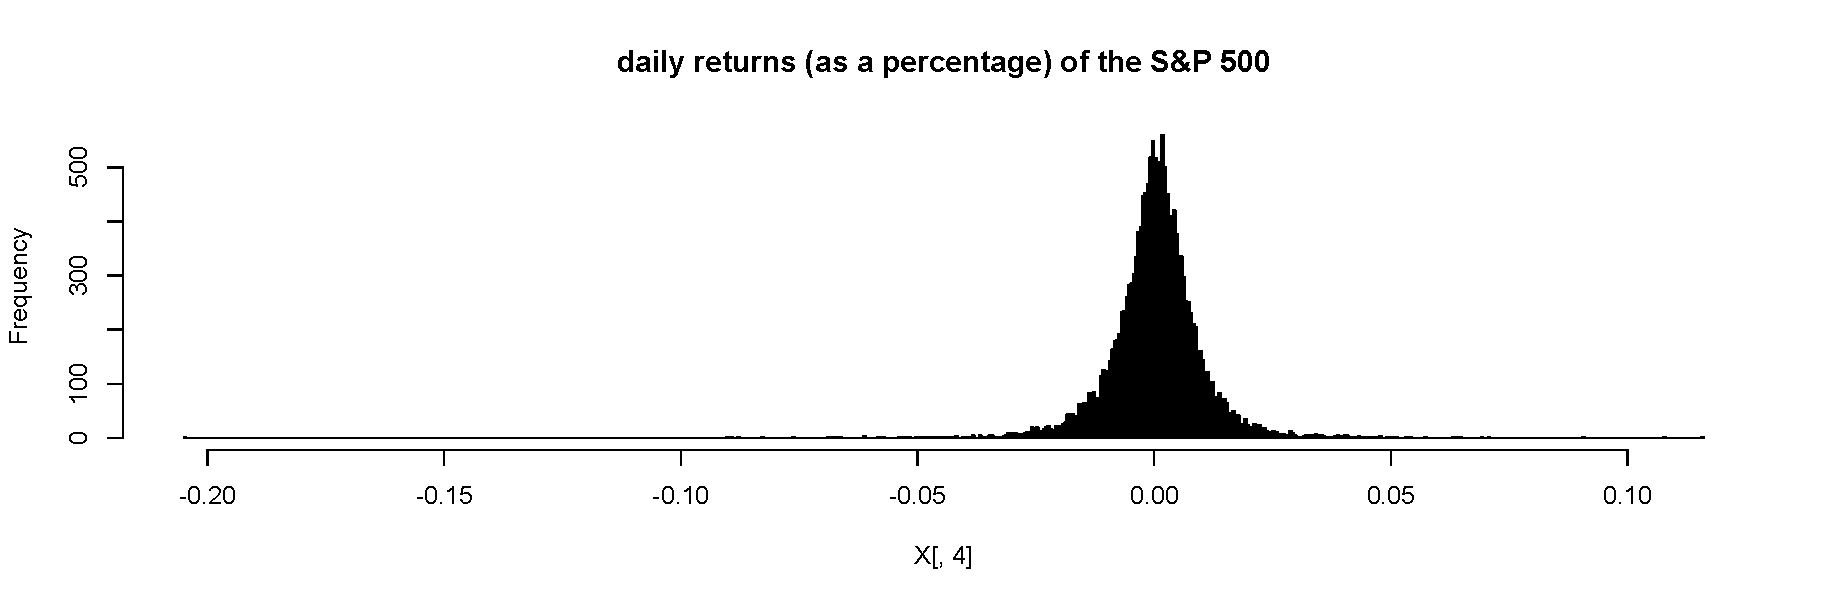
\includegraphics[width=7in]{daily_returns}
\end{figure}

%\begin{verbatim}
%X = read.csv('sp_tot_ret_price_1950.csv')
%n = nrow(X)
%n
%hist(X[,4], br = 1000, 
%  main = 'daily returns (as a percentage) of the S&P 500')
%\end{verbatim}

\intermediatesubproblem{Do you think the data is $\iid$? Explain.}\spc{1}

\intermediatesubproblem{Assume $\iid$ normal data regardless of what you wrote in (a) and (b). The sample average is $\xbar = 0.0003415$ and the sample standard deviation is $s = 0.0096$. Under an objective prior, give a 95\% credible region for the true mean daily return.}\spc{4}

\hardsubproblem{Give a 95\% credible region for \emph{tomorrow's} return using functions in Table~\ref{tab:eqs}.}\spc{4}

\end{enumerate}


\end{document}











